\section{Overview}

The CLAS12 spectrometer has been designed and built for the comprehensive experimental studies of matter, using primarily a high energy electron beam, \cite{youris}. Due to the experiments with which this spectrometer is involved it must be capable of detecting scattered electrons within the entirety of its acceptance range and at the highest possible efficiency with low background. The High Threshold Cerenkov Counter (see Fig.\ref{fig:setup}) in CLAS12 exists to fulfill such a goal---to detect scattered electrons in conjunction with the other systems and to generate a fast trigger signal. 
\begin{figure}[h]
    \centering
    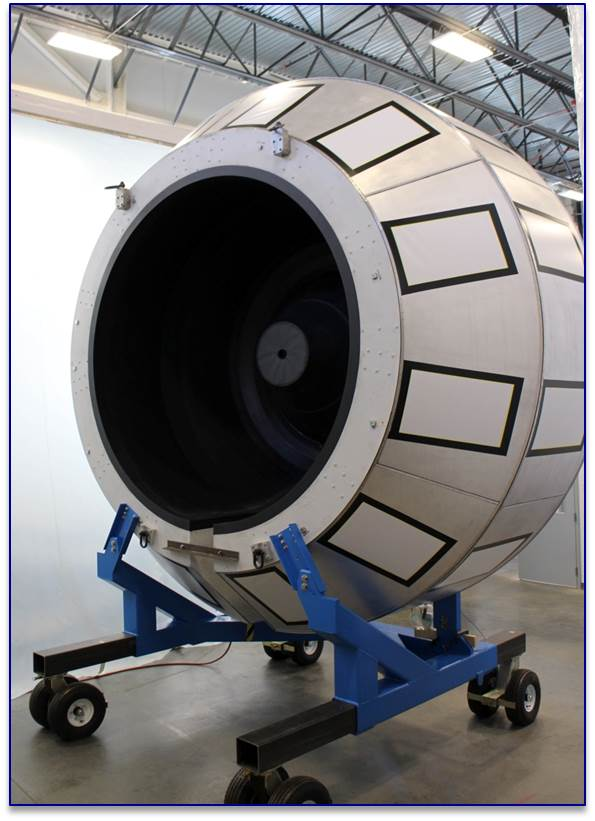
\includegraphics[width=0.75\linewidth]{Picture1.jpg}
    \caption{Assembled High Threshold Cerenkov Counter (HTCC)}
    \label{fig:setup}
\end{figure}{}
The distinguishing features of the detector were influenced by its location in front of the drift chambers. 

\begin{comment}
\begin{figure}[h]
    \centering
    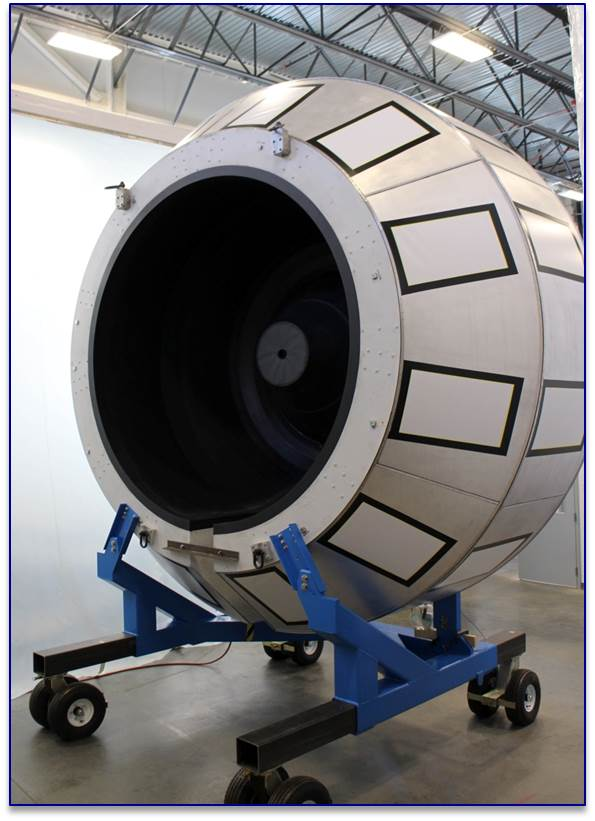
\includegraphics[width=0.75\linewidth]{Picture1.jpg}
    \caption{Caption}
    \label{fig:setup}
\end{figure}{}
\end{comment}

Its location required that the HTCC incorporate a minimum amount of material in front of the tracking detectors and, because the HTCC is a single module system, it uses very limited space inside of CLAS12. Consequently, the construction requirements---including transportation to the hall and installation into the nominal location of the detector---were all equally important for its structural design. 






